% Pengaturan ukuran teks dan bentuk halaman dua sisi
\documentclass[12pt]{report}

% Pengaturan ukuran halaman dan margin
\usepackage[a4paper,top=30mm,left=30mm,right=20mm,bottom=25mm]{geometry}

% Pengaturan ukuran spasi
\usepackage[singlespacing]{setspace}

% Pengaturan caption untuk tabel
\usepackage{caption}
\DeclareCaptionLabelSeparator{custom}{. }
\captionsetup
{
  labelsep = custom
}

% Judul dokumen
\title{Proposal Tugas Akhir ITS}
\author{Nirvana, Muhammad Naofal}

% Pengaturan detail pada file PDF
\usepackage[pdfauthor={\@author},bookmarksnumbered,pdfborder={0 0 0}]{hyperref}


% Pengaturan ukuran indentasi
\setlength{\parindent}{2em}

% Package lainnya
\usepackage{changepage}
\usepackage{etoolbox} % Mengubah fungsi default

% Pengaturan jenis karakter
\usepackage[utf8]{inputenc}

\usepackage[style=ieee, backend=biber]{biblatex}
\usepackage{enumitem} % Pembuatan list
\usepackage{lipsum} % Pembuatan template kalimat
\usepackage{graphicx} % Input gambar
\usepackage{longtable} % Pembuatan tabel
\usepackage[table,xcdraw]{xcolor} % Pewarnaan tabel
\usepackage{eso-pic} % Untuk menggunakan background image di halaman
\usepackage{txfonts} % Font times
\usepackage{changepage} % Pembuatan teks kolom
\usepackage{multicol} % Pembuatan kolom ganda
\usepackage{multirow} % Pembuatan baris ganda
\usepackage{tabularx} % Untuk mengatur kolom, seperti grid pada CSS
\usepackage{wrapfig}

% Pengaturan format daftar isi, daftar gambar, dan daftar tabel
\usepackage{tocloft}
\setlength{\cftbeforechapskip}{1.5ex}
\setlength{\cftbeforesecskip}{1.5ex}
\setlength{\cftbeforetoctitleskip}{0cm}
\setlength{\cftbeforeloftitleskip}{0cm}
\setlength{\cftbeforelottitleskip}{0cm}
\renewcommand{\cfttoctitlefont}{\hfill\Large\bfseries} % command untuk membuat heading bold dan besar
\renewcommand{\cftaftertoctitle}{\hfill}
\renewcommand{\cftloftitlefont}{\hfill\Large\bfseries}
\renewcommand{\cftafterloftitle}{\hfill}
\renewcommand{\cftlottitlefont}{\hfill\Large\bfseries}
\renewcommand{\cftafterlottitle}{\hfill}

% Definisi untuk "Hati ini sengaja dikosongkan"
\patchcmd{\cleardoublepage}{\hbox{}}{
  \thispagestyle{empty}
  \vspace*{\fill}
  \begin{center}\textit{[Halaman ini sengaja dikosongkan]}\end{center}
  \vfill}{}{}

  % Pengaturan penomoran halaman
\usepackage{fancyhdr}
\fancyhf{}
\renewcommand{\headrulewidth}{0pt}
\pagestyle{fancy}
\fancyfoot[R,RO]{\thepage}
\patchcmd{\chapter}{plain}{fancy}{}{}
\patchcmd{\chapter}{empty}{plain}{}{}

% Pengaturan format judul bab
\usepackage{titlesec}
\renewcommand{\thesection}{\thechapter.\arabic{section}}
\titleformat{\chapter}[hang]{\centering\bfseries\Large}{BAB\ \arabic{chapter}\ }{0ex}{\vspace{0ex}\centering}
\titleformat*{\section}{\large\bfseries}
\titleformat*{\subsection}{\normalsize\bfseries}
\titlespacing{\chapter}{0ex}{0ex}{4ex}
\titlespacing{\section}{0ex}{1ex}{1ex}
\titlespacing{\subsection}{0ex}{1ex}{1ex}
\titlespacing{\subsubsection}{0ex}{1ex}{1ex}
\setcounter{secnumdepth}{3} % Untuk memberi penomoran pada \subsubsection

\counterwithin{figure}{section}
\counterwithin{table}{section}

% Mengganti figure dan table menjadi gambar dan tabel
\renewcommand{\figurename}{Gambar}
\renewcommand{\tablename}{Tabel}

% Tambahkan format tanda hubung yang benar di sini
\hyphenation{
  ro-ket
  me-ngem-bang-kan
  per-hi-tu-ngan
}

% Menambahkan resource daftar pustaka
\addbibresource{pustaka/pustaka.bib}

% Isi keseluruhan dokumen
\begin{document}
% Nomor halaman pembuka dimulai dari sini
\pagenumbering{roman}

% Sampul Bahasa Indonesia
\newcommand\covercontents{sampul/konten-id.tex}
\AddToShipoutPictureBG*{
  \AtPageLowerLeft{
    % Ubah nilai berikut jika posisi horizontal background tidak sesuai
    \hspace{-3.25mm}

    % Ubah nilai berikut jika posisi vertikal background tidak sesuai
    \raisebox{0mm}{
      
\includegraphics[width=\paperwidth,height=\paperheight]{sampul/gambar/sampul-luar-tipis.png}
    }
  }
}

% Menyembunyikan nomor halaman
\thispagestyle{empty}

% Pengaturan margin untuk menyesuaikan konten sampul
\newgeometry{
  top=65mm,
  left=30mm,
  right=30mm,
  bottom=20mm
}

\begin{flushleft}

  % Pemilihan font sans serif
  \sffamily

  % Pemilihan font bold
  \fontseries{bx}
  \selectfont
  \begin{spacing}{1.5}
    \input{\covercontents}
  \end{spacing}

\end{flushleft}

\restoregeometry


% Sampul Bahasa Inggris
% \renewcommand\covercontents{sampul/konten-en.tex}
% \AddToShipoutPictureBG*{
  \AtPageLowerLeft{
    % Ubah nilai berikut jika posisi horizontal background tidak sesuai
    \hspace{-3.25mm}

    % Ubah nilai berikut jika posisi vertikal background tidak sesuai
    \raisebox{0mm}{
      
\includegraphics[width=\paperwidth,height=\paperheight]{sampul/gambar/sampul-luar-tipis.png}
    }
  }
}

% Menyembunyikan nomor halaman
\thispagestyle{empty}

% Pengaturan margin untuk menyesuaikan konten sampul
\newgeometry{
  top=65mm,
  left=30mm,
  right=30mm,
  bottom=20mm
}

\begin{flushleft}

  % Pemilihan font sans serif
  \sffamily

  % Pemilihan font bold
  \fontseries{bx}
  \selectfont
  \begin{spacing}{1.5}
    \input{\covercontents}
  \end{spacing}

\end{flushleft}

\restoregeometry


% Atur ulang penomoran halaman
\setcounter{page}{1}

% Lembar pengesahan
\addcontentsline{toc}{chapter}{LEMBAR PENGESAHAN}

\begin{center}
  \large
  \textbf{LEMBAR PENGESAHAN}
\end{center}

% Menyembunyikan nomor halaman
\thispagestyle{empty}

\begin{center}
  % Ubah kalimat berikut dengan judul tugas akhir
  \textbf{SISTEM PENDETEKSI PENGGUNAAN ALAT PELINDUNG DIRI (APD) PADA PEKERJA KONSTRUKSI}
\end{center}

\begingroup
% Pemilihan font ukuran small
\small

\begin{center}
  % Ubah kalimat berikut dengan pernyataan untuk lembar pengesahan
  \textbf{PROPOSAL TUGAS AKHIR} \\
  Diajukan untuk memenuhi salah satu syarat memperoleh gelar
  Sarjana Teknik pada
  Program Studi S-1 Teknik Komputer \\
  Departemen Teknik Komputer \\
  Fakultas Teknologi Elektro dan Informatika Cerdas \\
  Institut Teknologi Sepuluh Nopember
\end{center}

\begin{center}
  % Ubah kalimat berikut dengan nama dan NRP mahasiswa
  Oleh: \textbf{Muhammad Naofal Nirvana} \\
  NRP. 0721 19 4000 0066
\end{center}

\begin{center}
  Disetujui oleh Tim Penguji Proposal Tugas Akhir:
\end{center}

\begingroup
% Menghilangkan padding
\setlength{\tabcolsep}{0pt}

\noindent
\begin{tabularx}{\textwidth}{X c}
  % Ubah kalimat-kalimat berikut dengan nama dan NIP dosen pembimbing pertama
  Reza Fuad Rachmadi, S.T., M.T., Ph. D &                 \\
  NIP: 19850403 201212 1 001            & (Pembimbing I)  \\
                                        &                 \\
                                        &                 \\
  % Ubah kalimat-kalimat berikut dengan nama dan NIP dosen pembimbing kedua
  Dr. I Ketut Eddy Purnama, S.T., MT.   &                 \\
  NIP: 19690730 199512 1 001            & (Pembimbing II) \\
                                        &                 \\
                                        &                 \\
  % Ubah kalimat-kalimat berikut dengan nama dan NIP dosen penguji pertama
  % Dr. Galileo Galilei, S.T., M.Sc.  & (Penguji I) \\
  % NIP: 15640215 164201 1 001        & \\
                                        &                 \\
                                        &                 \\
  % Ubah kalimat-kalimat berikut dengan nama dan NIP dosen penguji kedua
  % Friedrich Nietzsche, S.T., M.Sc.  & (Penguji II) \\
  % NIP: 18441015 190008 1 001        & \\
                                        &                 \\
                                        &                 \\
  % Ubah kalimat-kalimat berikut dengan nama dan NIP dosen penguji ketiga
  % Alan Turing, ST., MT.             & (Penguji III) \\
  % NIP: 19120623 195406 1 001        & \\
\end{tabularx}
\endgroup

\vspace{4ex}

\begin{center}
  % Ubah text dibawah menjadi tempat dan tanggal
  \textbf{SURABAYA} \\
  \textbf{Desember, 2022}
\end{center}
\endgroup

\newpage

% Lembar pengesahan
% \begin{center}
  \large
  \textbf{APPROVAL SHEET}
\end{center}

% Menyembunyikan nomor halaman
\thispagestyle{empty}

\begin{center}
  % Ubah kalimat berikut dengan judul tugas akhir
  \textbf{PERSONAL PROTECTIVE EQUIPMENT (PPE) DETECTION SYSTEM ON CONSTRUCTION WORKERS}
\end{center}

\begingroup
% Pemilihan font ukuran small
\small

\begin{center}
  % Ubah kalimat berikut dengan pernyataan untuk lembar pengesahan
  \textbf{FINAL PROJECT PROPOSAL} \\
  Submitted to fulfill one of the requirements for obtaining the Bachelor of Engineering degree
  at Undergraduate Study Program of Computer Engineering \\
  Department of Computer Engineering \\
  Faculty of Intelligent Electrical and Informatcis Technology \\
  Sepuluh Nopember Institute of Technology
\end{center}

\begin{center}
  % Ubah kalimat berikut dengan nama dan NRP mahasiswa
  By: \textbf{Muhammad Naofal Nirvana} \\
  NRP. 0721 19 4000 0066
\end{center}

\begin{center}
  Approved by Final Project Proposal Examiner Team:
\end{center}

\begingroup
% Menghilangkan padding
\setlength{\tabcolsep}{0pt}

\noindent
\begin{tabularx}{\textwidth}{X c}
  % Ubah kalimat-kalimat berikut dengan nama dan NIP dosen pembimbing pertama
  Reza Fuad Rachmadi, S.T., M.T., Ph. D &              \\
  NIP: 19850403 201212 1 001            & (Advisor I)  \\
                                        &              \\
                                        &              \\
  % Ubah kalimat-kalimat berikut dengan nama dan NIP dosen pembimbing kedua
  Dr. I Ketut Eddy Purnama, ST., MT.    &              \\
  NIP: 19690730 199512 1 001            & (Advisor II) \\
                                        &              \\
                                        &              \\
  % Ubah kalimat-kalimat berikut dengan nama dan NIP dosen penguji pertama
  % Dr. Galileo Galilei, S.T., M.Sc.  &  \\
  % NIP: 15640215 164201 1 001        & (Examiner I) \\
                                        &              \\
                                        &              \\
  % Ubah kalimat-kalimat berikut dengan nama dan NIP dosen penguji kedua
  % Friedrich Nietzsche, S.T., M.Sc.  &  \\
  % NIP: 18441015 190008 1 001        & (Examiner II)\\
                                        &              \\
                                        &              \\
  % Ubah kalimat-kalimat berikut dengan nama dan NIP dosen penguji ketiga
  % Alan Turing, ST., MT.             &  \\
  % NIP: 19120623 195406 1 001        & (Examiner III)\\
\end{tabularx}
\endgroup

\vspace{4ex}

\begin{center}
  % Ubah text dibawah menjadi tempat dan tanggal
  \textbf{SURABAYA} \\
  \textbf{December, 2022}
\end{center}
\endgroup

% \newpage

% Abstrak
\addcontentsline{toc}{chapter}{ABSTRAK}
\begin{center}
  \large
  \textbf{ABSTRAK}
\end{center}

\begin{center}
  \large
  \textbf{SISTEM PENDETEKSI PENGGUNAAN ALAT PELINDUNG DIRI (APD) PADA PEKERJA KONSTRUKSI}
\end{center}

% Menyembunyikan nomor halaman
% \thispagestyle{empty}

\begin{flushleft}
  \setlength{\tabcolsep}{0pt}
  \bfseries
  \begin{tabular}{ll@{\hspace{6pt}}l}
    Nama Mahasiswa / NRP & : & Muhammad Naofal Nirvana / 0721 19 4000 0066 \\
    Departemen           & : & Teknik Komputer FTEIC - ITS                 \\
    Dosen Pembimbing     & : & 1. Reza Fuad Rachmadi, S.T., M.T., Ph. D    \\
                         &   & 2. Dr. I Ketut Eddy Purnama, ST., MT.       \\
  \end{tabular}
  \vspace{4ex}
\end{flushleft}
\textbf{Abstrak}

% Isi Abstrak
Alat Pelindung Diri (APD) adalah suatu alat yang mempunyai kemampuan untuk melindungi seseorang yang fungsinya mengisolasi sebagian atau seluruh tubuh dari potensi bahaya di tempat kerja. Terdapat peraturan yang menyatakan pentingnya dan mewajibkan penggunaan Alat Pelindung Diri seperti Peraturan Menteri Tenaga Kerja RI NOMOR PER.08/MEN/VII/2010 tentang PERATURAN ALAT PELINDUNG DIRI. Meskipun sudah diwajibkan dan diatur dalam peraturan menteri, tidak menjamin semua pekerja lapangan akan memakai APD tersebut. Perusahaan yang mengerjakan proyek konstruksi biasanya sudah mengerahkan pengawas untuk memastikan semua pekerja memakai APD yang sesuai ketentuan. Penempatan staf pengawas sendiri juga sudah diatur dalam salah satu peraturan Kementerian Ketenagakerjaan Republik Indonesia. Namun metode pengawasan yang digunakan masih dilakukan secara manual oleh staf-staf pengawas yang masih memiliki keterbatasan. Luasnya area lokasi kontstruksi dan jumlah pekerja yang sangat banyak menjadi tantangan tersendiri bagi staf pengawas sebagai seorang manusia untuk menjalankan tugasnya mengawasi setiap pekerja yang ada di area tersebut. Oleh karena itu, penelitian ini bertujuan untuk merancang suatu sistem yang bisa mendeteksi secara otomatis pekerja yang memakai APD lengkap dan yang memakai APD tidak lengkap serta memicu semacam alarm ketika sistem mendeteksi pekerja yang memakai APD yang tidak lengkap. Pengembangan sistem akan memanfaatkan \emph{Convolutional Neural Network} dan algoritma deteksi objek YOLOv7.

\vspace{2ex}
\noindent
\textbf{Kata Kunci: \emph{Alat Pelindung Diri, Sistem, Mendeteksi, Convolutional Neural Network}}
\newpage

\begin{center}
  \large
  \textbf{DETECTION SYSTEM OF PERSONAL PROTECTIVE EQUIPMENT (PPE) ON CONSTRUCTION WORKERS}
\end{center}
% Menyembunyikan nomor halaman
\thispagestyle{empty}

\begin{flushleft}
  \setlength{\tabcolsep}{0pt}
  \bfseries
  \begin{tabular}{lc@{\hspace{6pt}}l}
    Student Name / NRP & : & Muhammad Naofal Nirvana / 0721 19 4000 0066 \\
    Department         & : & Computer Engineering ELECTICS - ITS         \\
    Advisor            & : & 1. Reza Fuad Rachmadi, S.T., M.T., Ph. D    \\
                       &   & 2. Dr. I Ketut Eddy Purnama, ST., MT.       \\
  \end{tabular}
  \vspace{4ex}
\end{flushleft}
\textbf{Abstract}

% Isi Abstrak
Personal Protective Equipment (PPE) is a tool that has the ability to protect someone whose function is to isolate part or all of the body from potential hazards in the workplace. There are regulations that state the importance of and require the use of Personal Protective Equipment such as Regulation of the Minister of Manpower of the Republic of Indonesia NUMBER PER.08/MEN/VII/2010 concerning REGULATIONS FOR PERSONAL PROTECTIVE EQUIPMENT. Even though it is mandatory and regulated in a ministerial regulation, it does not guarantee that all field workers will wear the PPE. Companies working on construction projects usually have dispatched supervisors to ensure that all workers are wearing appropriate PPE. The placement of the supervisory staff itself has also been regulated in one of the regulations of the Ministry of Manpower of the Republic of Indonesia. However, the monitoring method used is still carried out manually by supervisory staff who has its limitations. The large area of the construction site and the large number of workers is a challenge for the supervisory staff as a human being to carry out their duties of supervising every worker in the area. Therefore, this study aims to design a system that can automatically detect workers wearing appropriate PPE and those wearing inappropriate PPE and triggering an alarm when the system detects workers wearing inappropriate PPE. System development will utilize the Convolutional Neural Network and the YOLOv7 object detection algorithm.

\vspace{2ex}
\noindent
\textbf{Keywords: \emph{Personal Protective Equipment, System, Detect, Convolutional Neural Network}}
\newpage

\begin{spacing}{1.5}
  % Daftar isi
  \renewcommand*\contentsname{DAFTAR ISI}
  \addcontentsline{toc}{chapter}{\contentsname}
  \tableofcontents
  \newpage

  % Daftar gambar
  \renewcommand*\listfigurename{DAFTAR GAMBAR}
  \addcontentsline{toc}{chapter}{\listfigurename}
  \listoffigures
  \newpage

  % Daftar tabel
  \renewcommand*\listtablename{DAFTAR TABEL}
  \addcontentsline{toc}{chapter}{\listtablename}
  \listoftables
  \newpage
\end{spacing}

% Nomor halaman isi dimulai dari sini
\pagenumbering{arabic}

% Konten pendahuluan
\section{PENDAHULUAN}

\subsection{Latar Belakang}

% Ubah paragraf-paragraf berikut sesuai dengan latar belakang dari tugas akhir
Pesatnya perkembangan roket yang merupakan \lipsum[2]

\lipsum[3]

\subsection{Rumusan Masalah}

% Ubah paragraf berikut sesuai dengan rumusan masalah dari tugas akhir
Berdasarkan hal yang telah dipaparkan di latar belakang, \lipsum[4]

\subsection{Batasan Masalah atau Ruang Lingkup}

\lipsum[6]

\subsection{Tujuan}

% Ubah paragraf berikut sesuai dengan tujuan penelitian dari tugas akhir
Tujuan dari penelitian ini adalah \lipsum[7][1-14]

\subsection{Manfaat}

% Ubah paragraf berikut sesuai dengan tujuan penelitian dari tugas akhir
Manfaat dari penelitian ini adalah \lipsum[8][1-14]


% Konten tinjauan pustaka
\section{TINJAUAN PUSTAKA}

% Ubah konten-konten berikut sesuai dengan isi dari tinjauan pustaka
\subsection{Hasil penelitian/perancangan terdahulu}

\subsubsection{\emph{PPE detector: a YOLO-based architecture to detect personal protective equipment (PPE) for construction Sites}}
Md. Ferdous dan Sk. Md. Masudul Ahsan pada bulan April 2022 lalu melakukan penelitian berjudul "PPE detector: a YOLO-based architecture to detect personal protective equipment (PPE) for construction Sites" dimana mereka membuat sistem pendeteksi APD otomatis berbasis Visi Komputer. Sedangkan untuk algoritma deteksi yang digunakan, penelitian ini menggunakan arsitektur \emph{anchor-free} YOLO --- yaitu YOLO versi X atau YOLOX secara spesifik. Penelitian ini menggunakan dataset bernama "CHVG Dataset" dimana CHVG merupakan kependekan dari \emph{Color Hardhat Vest Glass} yang merupakan deskripsi dari isi dari dataset itu sendiri. Dataset tersebut merupakan salah satu \emph{output} dari penelitian ini yang dibuat sendiri oleh para penulis dengan cara menambahkan dan menggabungkan data dari dataset penelitian-penelitian sebelumnya yang terkait serta sebagai pengembangan dari dataset penelitian-peneli- tian sebelumnya tersebut. Sistem deteksi yang dibuat oleh penelitian ini masih menerima \emph{input} dalam bentuk file gambar atau foto dan belum \emph{real-time} menggunakan kamera webcam yang menangkap citra video namun hasil prediksi dari model YOLOX sudah ditampilkan pada antarmuka sistem. Dari hasil pengujian yang dilakukan, didapatkan rata-rata mAP terbesarnya yaitu 89,84\% yang dihasilkan oleh model dengan jenis YOLOX-m \cite{ferdous_ahsan_2022}.

\subsubsection{Rancang Sistem Pendeteksi Alat Pelindung Diri (APD) Berbasis \emph{Image Prosessing}}

Miftachul Ulum bersama 3 rekannya pada tahun 2021 melakukan penelitian tentang peran-
cangan sistem pendeteksi Alat Pelindung Diri (APD) antara lain helm, kacamata, dan masker
dengan menerapkan metode CNN yang berbasis image processing. Sistem deteksi yang dirancang pada penelitian ini masih menerima input hanya dalam bentuk file gambar (tidak \emph{real-time}) yang berasal dari hasil tangkapan citra webcam. Selain itu hasil prediksi dari model yang digunakan tidak divisualisasikan langsung pada antarmuka sistem dan hanya bergantung pada \emph{buzzer} yang sudah diprogram untuk menyala jika terdeteksi APD tidak lengkap.
Dari hasil pengujian, didapatkan akurasi keberhasilan 75\% dengan klasifikasi objek yang menggunakan APD lengkap,
APD tidak lengkap, dan tidak menggunakan APD. Pada penelitian ini ditemukan bahwa kom-
ponen APD kacamata lebih sering tidak terdeteksi dibanding komponen APD lainnya yang
disebabkan oleh pantulan cahaya dari kacamata yang dapat mengganggu proses penangkapan gambar. Selain itu pada penelitian ini juga ditemukan bahwa kemampuan kamera dan komputer
akan memengaruhi kinerja sistem secara keseluruhan \cite{miftachul_2021}.

\subsection{Teori/Konsep Dasar}

\subsubsection{Alat Pelindung Diri}
\label{apd}

Dalam setiap pekerjaan, seorang pekerja memiliki kemungkinan mengalami kecelakaan yang mempengaruhi kondisi kesehatannya. Keselamatan dan kesehatan kerja berkaitan dengan alat kerja, proses pengolahan, dan bahan, lingkungan kerja dan proses melakukan pekerjaannya. Kecelakaan merupakan kejadian yang tidak terduga dan tidak pernah diharapkan karena dapat menimbulkan kerugian materil dan juga penderitaan mulai dari penderitaan yang ringan sampai dengan penderitaan yang paling berat \cite{anizar2012}.

Seperti diketahui, ada 5 tahapan yang mencakup upaya pencegahan kecelakaan dalam hierarki pengendalian risiko, yaitu: tahap eliminasi, substitusi, tahap engineering, tahap administrasi dan terakhir alat pelindung diri. Penggunaan alat ini bukanlah pilihan pertama melainkan yang terakhir jika 4 langkah tersebut belum dilakukan atau telah dilakukan namun masih terdapat bahaya yang mengganggu status kesehatan tenaga kerja. Penggunaan alat ini akan menimbulkan ketidaknyamanan pekerja namun mampu mencegah atau mengurangi resiko penyakit akibat kerja dan kecelakaan kerja \cite{k3ptglobal}.

Alat Pelindung Diri selanjutnya disingkat APD adalah
suatu alat yang mempunyai kemampuan untuk melindungi
seseorang yang fungsinya mengisolasi sebagian atau
seluruh tubuh dari potensi bahaya di tempat kerja.
Penggunaan APD diatur dalam Peraturan Menteri Tenga Kerja
dan Transmigrasi Republik Indonesia NOMOR PER.08/MEN/VII/2010
tentang ALAT PELINDUNG DIRI (dan Transmigrasi Republik Indonesia, 2010a) \cite{suratkementriantenagakerja}.

\newpage

\subsubsection{Peraturan Menteri Tenaga Kerja dan Transmigrasi Republik Indonesia tentang Alat Pelindung Diri}
\label{peraturanapd}

Peraturan Menteri Tenaga Kerja dan Transmigrasi (Kemnakertrans) Republik Indonesia NOMOR PER.08/MEN/VII/2010 mengatur tentang alat pelindung diri.
Peraturan ini meliputi pihak - pihak yang terlibat, kewajiban penyediaan APD, peralatan yang termasuk APD, dan karakteristik tempat
yang diwajibkan APD \cite{suratkementriantenagakerja}. Pada pasal 3 ayat 1, disebutkan alat - alat yang termasuk sebagai alat pelindung diri
yaitu :

\begin{enumerate}[nolistsep]
  \item pelindung kepala
  \item pelindung mata dan muka
  \item pelindung telinga
  \item pelindung pernapasan beserta kelengkapannya
  \item pelindung tangan
  \item pelindung kaki
\end{enumerate}

\subsubsection{Peraturan Menteri Pekerjaan Umum dan Perumahan Rakyat tentang Pedoman Sistem Manajemen Keselamatan Konstruksi}
\label{sec:permenpu_smkk}

\par Peraturan Menteri Pekerjaan Umum dan Perumahan Rakyat NOMOR : 21/PRT/M/2019 mengatur Pedoman Sistem Manajemen Keselamatan Konstruksi.
Petaturan ini meliputi ketentuan umum untuk SMKK (Sistem Manajemen Keselamatan Konstruksi), Konseptual SMKK, elemen SMKK, penerapan, penyedia jasa, pelaksanaan pekerjaan konstruksi,  dan beberapa aturan lainnya yang menyinggung ketentuan Kesehatan Keselamatan Kerja (K3) pada konstruksi. Pada pasal 1 untuk ketentuan umum dimana pada ayat ke 10 menyebutkan adanya Pengawas Pekerjaan Konstruksi yang merupakan tim pendukung yang ditunjuk oleh Pengguna Jasa yang bertanggung jawab pada pengawasan Pekerjaan Konstruksi dan pemenuhan terhadap norma, standar, prosedur, dan kriteria \cite{permen21prtm2019pedomansistemmanajemenkeselamatankonstruksi}.

\subsubsection{Visi Komputer}
\label{sec:visikomputer}

\par Manusia bisa dengan mudahnya memahami struktur tiga dimensi yang ada di sekitarnya. Kita dapat mengetahui bahwa
sebuah balok memiliki ketebalan atau sebuah pot bunga yang memiliki isi. Kita juga dapat memahami benda yang semi transparan
seperti kantong plastik dimana cahaya matahari dapat menembus lembaran plastik tersebut. Lalu saat kita mengamati suatu kumpulan
barang - barang di gudang, kita juga dapat dengan mudahnya menentukan nama dari barang tersebut dan lokasinya. Begitu juga saat
mengamati foto keluarga yang terdiri dari banyak individu dimana kita dapat membedakan antara satu dengan yang lainnya bahkan hingga
emosi yang mereka perlihatkan lewat raut wajahnya. Peneliti sudah melakukan pengembangan untuk metode pengenalan visual seperti pada
manusia untuk komputer yang dimana bidangnya disebut sebagai \emph{Computer Vision} (Visi Komputer). Tetapi untuk mencapai titik dimana
komputer memiliki kemampuan untuk yang sama dengan manusia seperti dapat menghitung jumlah binatang yang ada dalam suatu gambar masih menjadi
sesuatu yang sulit. Hal ini dikarenakan bidang visi komputer ini merupakan bentuk \emph{inverse problem} dimana kita berusaha untuk menarik
suatu kesimpulan untuk suatu solusi tetapi informasi yang dimiliki sangat terbatas. Beberapa solusi yang memungkinkan untuk menyelesaiakan
permasalah visi komputer ini yaitu antaralain dengan penyelesaian secara fisika atau perhitungan probabilitas \cite{szeliski2010computer}.

\par Dalam visi komputer, kita berusaha untuk memahami dunia yang ditangkap dalam satu gambar atau lebih dan meniru ulang setiap detil nya seperti
bentuk, pencahayaan, dan pewarnaan. Manusia dapat dengan mudahnya memahami detail - detail tersebut sedangkan algoritma visi komputer
akan sering mengalami \emph{error} \cite{margaret2008mind}.

\newpage

\par Visi Komputer adalah bidang ilmu yang mempelajari cara untuk memproses gambar teru- tama dalam meniru
kemampuan manusia dalam melihat. Kemampuan seperti rekognisi wajah hingga bentuk kemampuan lain yang bahkan
melebihi kemampuan manusia. Kebanyakan riset dari bidang visi komputer di \emph{deep learning} berfokus pada
pengenalan objek atau deteksi. Bentuknya dari pengenalan atau deteksi ini bisa meliputi membuat log atau laporan
objek apa saja yang ada dalam gambar hingga memberi penandaan pada objek yang terdeteksi \cite{Goodfellow-et-al-2016}.

\subsubsection{\emph{Object Detection}}
\label{sec:objectdetection}

\par Untuk dapat memahami konsep deteksi objek, selain menyelesaikan klasifikasi kelas dari objek yang diamati, kita juga harus dapat
menentukan lokasi dari objek yang diamati secara akurat dalam gambar yang sedang diamati. Proses penentuan lokasi sekaligus menentukan
klasifikasi kelas untuk menentukan "nama" dari objek yang diamati inilah yang disebut sebagai \emph{Object Detection} \cite{felzenszwalb2010object}.

\par Manfaat dari \emph{Object Detection} yaitu dapat memberikan informasi terkait suatu gambar atau video agar bisa lebih dipahami yang lalu bisa dimanfaatkan
untuk berbagai bentuk aplikasi. Penelitian di bidang \emph{Object Detection} ini pada umumnya berjalan di area \emph{neural network} atau sistem \emph{machine learning}
yang lalu juga termasuk pembuatan algoritma \emph{neural network} untuk teknik deteksi objek. Tetapi deteksi pada suatu gambar memiliki banyak
hal yang perlu dipertimbangkan seperti arah sudut pandang, pencahayaan, objek yang menghalang, dan hal lainnya yang membuat
deteksi objek dengan prediksi lokasi akurat semakin sulit untuk dilakukan \cite{zhao2019object} \cite{girshick2014rich}.

\par Proses penyelesain deteksi objek biasanya dilakukan dalam 3 tahap yaitu pemilihan wila- yah informatif, ekstraksi fitur, dan
klasifikasi.

\par Ada kemungkinan bahwa terdapat lebih dari satu objek yang ada dalam satu gambar yang akan dilakukan proses deteksi objek dan
juga berkemungkinan memiliki ukuran yang berbeda - beda. Pada tahap inilah dilakukan pemilihan region atau wilayah dengan melakukan \emph{scanning} pada gambar tersebut mulai
dari bagian awal gambar hingga akhir yang dimana merupakan metode yang sangat menguras energi dan memiliki banyak kelemahan \cite{zhao2019object}.

\par Tahap ekstraksi fitur kelas berguna untuk membedakan objek - objek yang berbeda dari gambar yang sedang diamati dimana kita perlu
memilah - milah "fitur" visual yang dapat memberi kita informasi yang dapat diapahami. Terdapat beberapa metode berbeda yang dilakukan
untuk mendapatkan fitur yang membantu untuk mengenali objek tersebut seperti SIFT, HOG, dan Haar-like \cite{zhao2019object}. Tetapi pada \emph{Convolutional Neural Network}
proses ekstraksi fitur nya dilakukan pada \emph{neural network}-nya juga yang akan dijelaskan pada Subbab~\ref{sec:convolutionalneuralnetwork}.

\par Klasifikasi berguna untuk mengenali objek yang ada pada gambar dengan kategori - kategori. Juga sudah terdapat beberapa metode
klasifkasi yang biasa digunakan seperti \emph{Supported Vector Machine}, AdaBoost, dan \emph{Deformable Part-based Model} \cite{zhao2019object}.

\subsubsection{\emph{Convolutional Neural Network} (CNN)}
\label{sec:convolutionalneuralnetwork}

\par \emph{Convolutional Neural Network} adalah metode deep learning yang didesain untuk rekognisi pada data dua
dimensi yang dimana umumnya berupa gambar visual (tetapi tidak harus berupa gambar) dan untuk klasifikasi.
Convolutional Neural Network memiliki kedalaman jaringan yang tinggi sehingga juga bisa termasuk sebagai \emph{Deep Neural Network}.
Jika dibandingan dengan \emph{Multilayer Perceptron} atau MLP, kemampuan CNN untuk klasifikasi citra lebih baik dibandingkan dengan MLP karena MLP tidak memiliki
kemampuan untuk menyimpan \emph{spatial information} dari gambar dimana satu \emph{pixel} pada gambar dianggap sebagai satu fitur
terpisah atau independen \cite{putra2016klasifikasi}. \emph{Convolutional Neural Network} adalah bentuk \emph{deep neural network} yang tidak hanya
sekadar memiliki banyak \emph{layer} seperti konsep \emph{deep learning} tetapi juga meniru bagaimaimana cara otak manusia mengenali sebuah gambar \cite{kim2017convolutional}. Pada arsitektur CNN, terdapat beberapa jenis layer yaitu \emph{Convolution Layer, Subsampling Layer,
  Fully Connected Layer}, dan \emph{Activation Layer}.

\subsubsection{\emph{You Only Look Once} (YOLO)}
\label{sec:youonlylookone}

\emph{You Only Look Once} atau YOLO adalah algoritma \emph{multi object detection} yang sangat cepat yang dicetuskan oleh Redmot et al pada tahun 2015 lewat buku mereka \emph{You Only Look Once: Unified, Real-Time Object Detection} \cite{redmon2016you}. \emph{Convolutional Neural Network} menjadi basis dari sistem deteksi YOLO ini. YOLO melakukan deteksi objek dengan menganggap nya sebagai permasalahan regresi tunggal yang diambil langsung dari \emph{pixel - pixel} yang ada di gambar menjadi \emph{bounding box} penanda dari koordinat - koordinat dan probabilitas dari klasifikasinya. Dengan begitu hanya perlu dilakukan satu kali pengecekan pada gambar untuk melakukan deteksi atau indentifikasi \cite{redmon2016you}. YOLO menggabungkan beberapa komponen dari teksi objek menjadi satu neural network yang dimana menggunakan fitu-fitur dari seluruh bagian gambar untuk memprediksi tiap \emph{bounding box} sekaligus melakukan prediksi untuk semua \emph{bounding box} di semua tipe klasifikasi yang ada. Desain dari YOLO ini memungkinkan untuk melakukan \emph{end to end training} dan kecepatan deteksi \emph{real time}.

\par Model YOLO (You Only Look Once) adalah pendeteksi objek \textit{single stage}. Bingkai gambar ditampilkan melalui \emph{\textit{Backbone}}, fitur digabungkan dan dicampur di \emph{\textit{Neck}}, dan kemudian diteruskan ke \emph{\textit{Head}} jaringan di mana YOLO memprediksi lokasi \emph{\textit{bounding box}}, kelas \emph{\textit{bounding box}}, dan objek \emph{\textit{bounding box}}. YOLO menggunakan pasca-pemrosesan melalui NMS untuk sampai pada prediksi akhirnya. Struktur jaringan tersebut ditunjukkan pada Gambar~\ref{fig:strukturyolo} \cite{strukturyolo}.

\begin{figure}[ht]
  \centering
  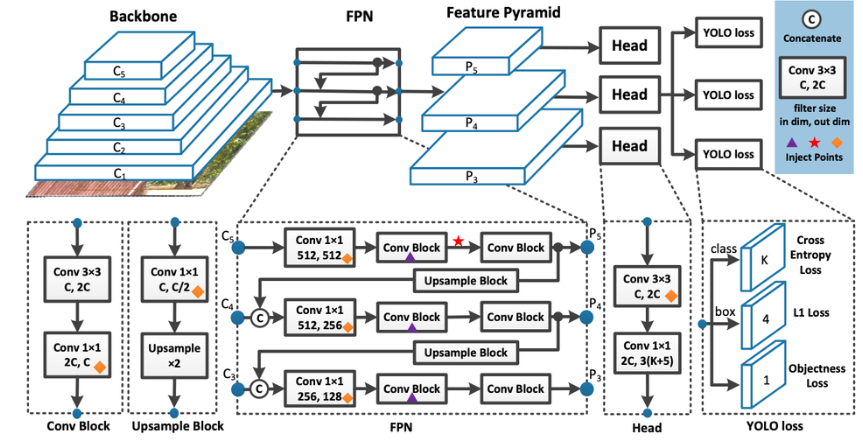
\includegraphics[width=0.85\textwidth]{gambar/arsitektur_yolo.png}
  \caption{Struktur Jaringan YOLO}
  \label{fig:strukturyolo}
\end{figure}

\par Sistem dari YOLO sendiri membagi input gambar menjadi grid S x S. Grid disini perannya untuk nanti yaitu jika grid tertentu menjadi pusat dari objek maka grid tersebut yang nantinya berguna untuk deteksi objek tadi.

\par Setiap grid memprediksi tiap bound box dan nilai kemungkinan klasifikasi atau \emph{confidence score} dari \emph{bounding box} tersebut. Nilai tersebut mewakili seberapa "yakin" model akan objek yang terdeteksi di bounding box dan seberapa akurat prediksinya.

\par Terdapat lima nilai prediksi yang ada pada tiap bounding box yaitu : x, y, w, h, dan \emph{confidence}. X dan Y mewakili pusat dari bounding box. W dan H mewakili \emph{Weight} dan \emph{Height} diprediksi relatif dari seluruh gambar. Lalu \emph{confidence score} sendiri mewakili IOU antara \emph{predicted box} dan \emph{ground truth box} \cite{redmon2016you}.

\subsubsection{YOLOv7}
\label{subsec:yolov7}

\par YOLOv7 adalah YOLO resmi versi terbaru yang dibuat oleh penulis asli arsitektur YOLO, melebihi semua versi YOLO sebelumnya dan model deteksi objek lainnya dalam hal kecepatan dan akurasi \cite{wang2022yolov7}. YOLOv7 meningkatkan kecepatan dan akurasi dengan memperkenalkan beberapa reformasi arsitektur. Mirip dengan \textit{Scaled} YOLOv4, YOLOv7 tidak menggunakan \textit{backbone pretrained} ImageNet. Sebaliknya, model dilatih menggunakan dataset COCO sepenuhnya. Kesamaan bisa diekspektasi karena YOLOv7 ditulis oleh penulis yang sama dari \textit{Scaled} YOLOv4 \cite{yolov7explain}.

Perubahan besar yang telah diperkenalkan pada makalah YOLOv7 salah satunya adalah reformasi arsitektur yaitu dengan adanya E-ELAN (\textit{Extended Efficient Layer Aggregation Network}) dan \textit{Model Scaling} untuk Model Berbasis Rangkaian. E-ELAN (\textit{Extended Efficient Layer Aggregation Network}) adalah blok komputasi di bagian \textit{Backbone} YOLOv7. Hal tersebut mendapatkan inspirasi dari penelitian sebelumnya tentang efisiensi jaringan. Ini telah dirancang dengan menganalisis faktor-faktor berikut yang memengaruhi kecepatan dan akurasi yaitu \textit{memory access cost, I/O channel ratio, element wise operation, activations}, dan \textit{gradient path}. Secara sederhana, arsitektur E-ELAN memungkinkan \textit{framework} untuk belajar lebih baik. Ini didasarkan pada blok komputasi ELAN \cite{yolov7explain}.

% Konten metodologi

\section{METODOLOGI}

% Ubah konten-konten berikut sesuai dengan isi dari metodologi

\subsection{Desain Sistem}
\label{sec:desainsistem}

Judul untuk tugas akhir “Sistem Pendeteksi Penggunaan Alat Pelindung Diri (APD) Pada Pekerja Konstruksi” ini berada dalam bidang computer vision atau visi komputer yang memiliki tujuan merancang sistem yang dapat mendeteksi penggunaan Alat Pelindung Diri (APD) secara real-time. Menggunakan YOLOv7 yang merupakan algoritma deteksi objek yang berbasis CNN (Convolutional Neural Network). Dataset yang digunakan berupa gambar-gambar personel proyek yang mengenakan Alat Pelindung Diri (APD) dan yang tidak. Gambar - gambar tersebut dikumpulkan dari beberapa sumber seperti dataset dari penelitian sebelumnya dan sumber lainnya.

\begin{figure}[ht]
  \centering
  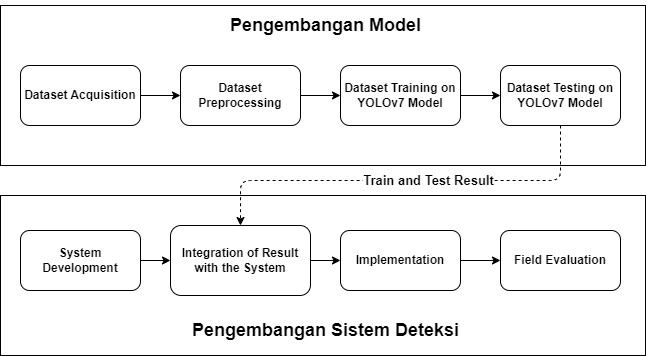
\includegraphics[width=1.0\textwidth]{gambar/desain_sistem.png}
  \caption{Bagan Umum Sistem}
  \label{fig:baganumumsistem}
\end{figure}

\newpage

\subsection{Akuisisi Dataset}
\label{sec:akuisisidataset}

Dataset yang digunakan untuk training menggunakan Yolov7 berupa dataset berisi gambar - gambar yang mengandung personel lapangan proyek yang mengenakan Alat Pelindung Diri (APD) dan yang tidak mengenakan APD. Untuk penelitian ini, dataset yang digunakan bersumber dari:

\subsubsection{CHVG Dataset oleh Md. Ferdous dan Sk. Md. Masudul Ahsan}
\label{chvgdataset}

\par Dataset ini merupakan dataset yang dibuat dan digunakan pada penelitian oleh Md. Ferdous dan Sk. Md. Masudul Ahsan pada bulan Juni tahun 2022 tentang sistem pendeteksi APD.
CHVG merupakan singkatan dari \textit{Color Hardhat, Vest, Glass} yang menggambarkan konten dari dataset itu sendiri. Dataset ini berisi delapan kelas yang berbeda, yaitu helm keselamatan kerja 4 warna (merah, biru, kuning, dan putih) dimana setiap warna memiliki kelasnya sendiri, rompi, kacamata pengaman, tubuh orang, dan kepala orang.
Dataset ini berisi 1.699 gambar dengan ukuran 640x640 dan anotasi yang sesuai dari delapan kelas tersebut \cite{Ferdous2022}.

\begin{figure}[ht]
  \centering
  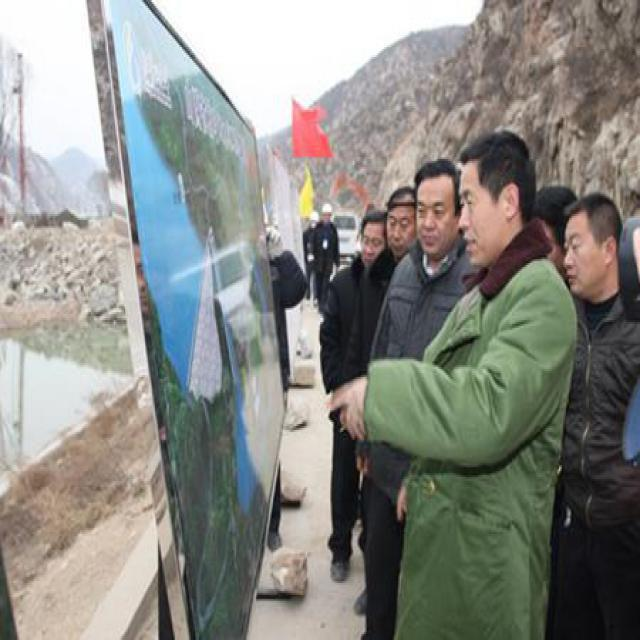
\includegraphics[width=0.3\textwidth]{gambar/chvg1}
  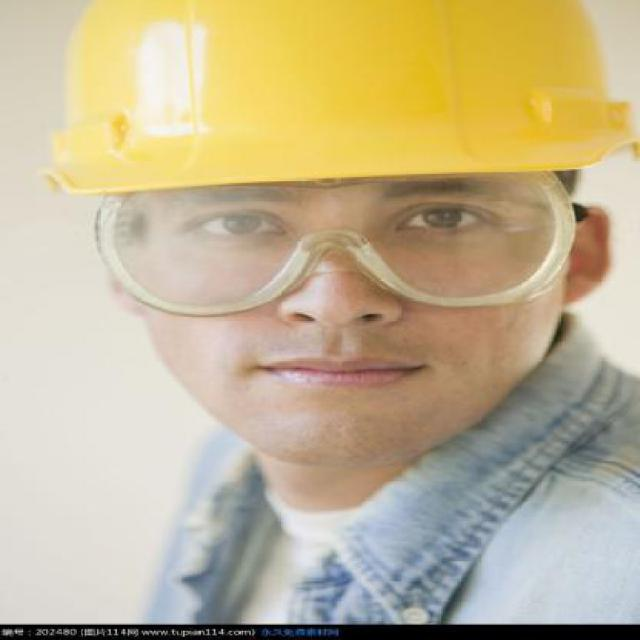
\includegraphics[width=0.3\textwidth]{gambar/chvg2}
  
\includegraphics[width=0.3\textwidth]{gambar/chvg3}
  \caption{Sampel gambar pada CHVG Dataset oleh Md. Ferdous dan Sk. Md. Masudul Ahsan}
  \label{fig:datasetapdpreview}
\end{figure}

\subsection{\textit{Preprocessing} Dataset}
\label{sec:preprocessing}
\par Ada beberapa proses yang dilakukan untuk dataset yang sudah dikumpulkan agar bisa digunakan untuk proses training dengan benar. Proses tersebut meliputi membersihkan dataset, augmentasi gambar, dan pembagian dataset. Untuk penelitian ini, proses - proses tersebut akan dilakukan pada platform Roboflow.

\subsection{Training dan Testing Model YOLOv7}
\label{sec:trainingdataset}

\par Dataset - dataset yang sudah di pre-process sebelumnya di roboflow dan sudah memiliki anotasi yang sesuai lalu digunakan untuk training model menggunakan algoritma YOLOv7. Training ini merupakan proses pelatihan model dengan input gambar - gambar dari dataset yang sudah diberi anotasi dimana gambar dan anotasinya tersebut diolah hingga menghasilkan suatu karakteristik atau pola khusus dari kelas/label yang ditentukan sebelumnya lewat anotasi sehingga selanjutnya dapat digunakan komputer untuk menebak gambar yang nantinya dideteksi. Karena YOLOv7 yang menggunakan PyTorch sebagai framework machine learningnya, hasil training nya berupa bobot atau weight yang akan diexport dalam bentuk .pt (format pytorch).

\par Hasil training model YOLOv7 tersebut kemudian dilakukan testing dengan cara melakukan proses \textit{inference} dimana input gambar yang digunakan merupakan gambar-gambar dari dataset itu sendiri yang sebelumnya digunakan untuk proses training.

\subsection{Pengembangan Sistem}
\label{sec:pengembangansistem}

Sistem deteksi Alat Pelindung Diri (APD) ini akan memanfaatkan YOLOv7 untuk melaku- kan prediksi pada input yang diterima. Input berupa gambar yang diterima dari
webcam atau camera yang terhubung ke komputer yang akan menjalankan sistem ini.
Sistem dikembangkan dengan tujuan untuk mendeteksi penggunaan Alat Pelindung Diri (APD) secara real-time dan akan menjalankan mekanisme alarm jika pada camera input
terdapat seseorang yang tidak menggunakan Alat Pelindung Diri (APD) secara lengkap. Dalam hal ini yaitu menggunakan helm, kacamata, dan rompi.

Sistem akan dibuat dalam bentuk file script python yang dapat dijalankan pada device komputer atau laptop. Script ini akan menerima beberapa parameter input yang dibutuhkan untuk menjalankan prediksi dengan model YOLOv7. Parameter input yang dibutuhkan yaitu salah satunya input feed camera dari webcam yang digunakan atau bisa dalam bentuk file gambar atau video.
Selain itu user akan harus memberikan parameter-parameter lain secara manual yang dibutuhkan model YOLOv7 agar dapat bisa menjalankan prediksi. Setelah semua parameter telah dipenuhi, sistem akan memberikan output berupa \textit{bounding box} yang meng-\textit{highlight} komponen-komponen APD yang ada pada gambar.

\subsection{Integrasi Sistem dengan Hasil Training Model}
\label{subsec:integrasi}

Sistem deteksi yang sudah dikembangkan akan diintegrasikan dengan model YOLOv7 yang sudah dilakukan training dan testing menggunakan CHVG dataset. Setelah diintegrasikan, sistem akan siap untuk diimplementasikan secara real-time dengan memanfaatkan input dari kamera webcam.

\subsection{Implementasi}
\label{subsec:implementasi}

Sistem deteksi yang sudah dilakukan integrasi selanjutnya akan diimplementasikan dimana sistem digunakan pada kondisi \textit{real-time}. Kamera webcam akan diarahkan kepada orang yang menggunakan maupun tidak menggunakan Alat Pelindung Diri (APD). Proses ini dilakukan berulang kali dengan beberapa variabel yang berbeda contohnya seperti kondisi gelap, berkabut, dan hujan.

\subsection{Evaluasi}
\label{subsec:evaluasi}

Setelah sistem deteksi diimplementasikan secara \emph{real-time} dengan beberapa variabel yang berbeda, dilakukan analisa hasil sebagai evaluasi sistem dan penelitian secara kesuluruhan. Setiap hasil dari variabel-variabel yang diuji akan dibandingkan untuk setiap jenis percobaan.

\subsection{Bahan dan peralatan yang digunakan}
\label{subsec:peralatan}

Dalam penelitian ini, bahan dan peralatan yang akan digunakan dalam rangka menyelesaikan penelitian ini mulai dari tools berupa software atau perangkat lunak hingga hardware atau perangkat keras. Berikut pemaparan dari alat-alat yang digunakan.

\begin{enumerate}[nolistsep]
  \item Computer Desktop
  \item Google Colab
  \item Webcam Papalook PA552pro
\end{enumerate}

\begin{longtable}{|c|c|c|}
  \caption{Spesifikasi Komputer Desktop}
  \label{tb:spesifikasikomputer}                         \\
  \hline
  % \rowcolor[HTML]{C0C0C0}
  \textbf{Tipe}      & \textbf{Detail}                   \\
  \hline
  \textit{Processor} & AMD Ryzen 3 3300X                 \\
  Memory             & 16 GB                             \\
  Storage            & HDD 1TB SSD 512GB                 \\
  Graphic Card       & NVIDIA GeForce GTX 1650 Super 4GB \\
  Operating System   & Windows 11                        \\
  CUDA               & CUDA version 11.8                 \\
  \hline
\end{longtable}

\begin{longtable}{|c|c|c|}
  \caption{Spesifikasi Webcam Papalook PA552pro}
  \label{tb:spesifikasiwebcam}                           \\
  \hline
  % \rowcolor[HTML]{C0C0C0}
  \textbf{Tipe} & \textbf{Detail}                        \\
  \hline
  Resolution    & 1920x1080                              \\
  Max FPS       & 60 FPS                                 \\
  Other Detail  & Full 360 Degree Rotation               \\
                & Auto Focus                             \\
                & Auto Exposure White Balance            \\
                & 3 Level Lighting Adjustable Ring Light \\
  \hline
\end{longtable}

\newpage

\subsection{Urutan pelaksanaan penelitian}

Alur waktu penelitian yang akan dilaksanakan akan mengacu pada tabel yang ditunjukkan pada Tabel~\ref{tb:timeline}.

% Ubah tabel berikut sesuai dengan isi dari rencana kerja
\newcommand{\w}{}
\newcommand{\G}{\cellcolor{gray}}
\begin{table}[h!]
  \caption{\emph{Timeline} Penelitian}
  \label{tb:timeline}

  \begin{tabular}{|p{3.5cm}|c|c|c|c|c|c|c|c|c|c|c|c|c|c|c|c|}
    \hline
    \multirow{2}{*}{Kegiatan} & \multicolumn{16}{|c|}{Minggu}                                                                       \\
    \cline{2-17}              &
    1                         & 2                             & 3  & 4  & 5  & 6  & 7  & 8  & 9  & 10 & 11 & 12 & 13 & 14 & 15 & 16 \\
    \hline

    % Gunakan \G untuk mengisi sel dan \w untuk mengosongkan sel
    Studi Literatur           &
    \G                        & \G                            & \G & \G & \w & \w & \w & \w & \w & \w & \w & \w & \w & \w & \w & \w \\
    \hline

    Pengolahan Data           &
    \w                        & \w                            & \G & \G & \G & \G & \w & \w & \w & \w & \w & \w & \w & \w & \w & \w \\
    \hline

    Training dan Testing      &
    \w                        & \w                            & \w & \w & \w & \G & \G & \G & \G & \w & \w & \w & \w & \w & \w & \w \\
    \hline

    Pengembangan Sis- tem     &
    \w                        & \w                            & \w & \w & \G & \G & \G & \G & \G & \w & \w & \w & \w & \w & \w & \w \\
    \hline

    Integrasi Sistem          &
    \w                        & \w                            & \w & \w & \w & \w & \w & \w & \w & \G & \G & \w & \w & \w & \w & \w \\
    \hline

    Implementasi              &
    \w                        & \w                            & \w & \w & \w & \w & \w & \w & \w & \w & \w & \G & \G & \G & \G & \w \\
    \hline

    Evaluasi                  &
    \w                        & \w                            & \w & \w & \w & \w & \w & \w & \w & \w & \w & \w & \w & \w & \G & \G \\
    \hline

    Pembuatan Laporan         &
    \G                        & \G                            & \G & \G & \G & \G & \G & \G & \G & \G & \G & \G & \G & \G & \G & \G \\
    \hline
  \end{tabular}
\end{table}

% Konten lainnya
\section{HASIL YANG DIHARAPKAN}

\subsection{Hasil yang Diharapkan dari Penelitian}

\par Hasil yang diharapkan dari penelitian ini adalah sistem pendeteksi penggunaan Alat Pelindung Diri (APD) pada pekerja konstruksi ini dapat diimplementasikan secara \emph{real-time} di lokasi kontstruksi dan membantu proses pengawasan yang dilakukan oleh staf pengawas K3 di lapangan. Selain itu, dengan adanya sistem ini penulis juga berharap akan meningkatkan kedisiplinan pemakaian APD oleh pekerja konstruksi sehingga mengurangi kemungkinan cedera, sakit, maupun kematian di lokasi konstruksi jika terjadi kecelakaan kerja.

\subsection{Hasil Pendahuluan}

\lipsum[16]


% Daftar pustaka
\chapter*{DAFTAR PUSTAKA}
\addcontentsline{toc}{chapter}{DAFTAR PUSTAKA}
\renewcommand\refname{}
\vspace{2ex}
\renewcommand{\bibname}{}
\begingroup
\def\chapter*#1{}
\printbibliography
\endgroup


\end{document}
